\hypertarget{political-alignment-and-polarization}{%
\chapter{Political Alignment and
Polarization}\label{political-alignment-and-polarization}}

This chapter and the next make up a case study that uses data from the
General Social Survey (GSS) to explore political beliefs and political
alignment (conservative, moderate, or liberal) in the United States.

In this chapter, we:

\begin{enumerate}
\def\labelenumi{\arabic{enumi}.}
\item
  Compare the distributions of political alignment from 1974 and 2021.
\item
  Plot the mean and standard deviation of responses over time as a way
  of quantifying shifts in political alignment and polarization.
\item
  Use local regression to plot a smooth line through noisy data.
\item
  Use cross tabulation to compute the fraction of respondents in each
  category over time.
\item
  Plot the results using a custom color palette.
\end{enumerate}

As an exercise, you will look at changes in political party affiliation
over the same period.

In the next chapter, we'll use the same dataset to explore the
relationship between political alignment and other attitudes and
beliefs.

In the the repository for this book, you'll find an HDF file that
contains the GSS data, which I have cleaned and resampled to correct for
stratified sampling. The file that contains three resamplings; we'll use
the first, \passthrough{\lstinline!gss0!}, to get started.

\begin{lstlisting}[]
datafile = "gss_pacs_resampled.hdf"
gss = pd.read_hdf(datafile, "gss0")
gss.shape
(@\dashfill@)
@@@(68846, 204)@@@
\end{lstlisting}

\hypertarget{political-alignment}{%
\section{Political Alignment}\label{political-alignment}}

The people surveyed as part of the GSS were asked about their
``political alignment'', which is where they place themselves on a
spectrum from liberal to conservative.

The variable \passthrough{\lstinline!polviews!} contains responses to
the following question (see
\url{https://gssdataexplorer.norc.org/variables/178/vshow}):

\begin{quote}
We hear a lot of talk these days about liberals and conservatives. I'm
going to show you a seven-point scale on which the political views that
people might hold are arranged from extremely liberal--point 1--to
extremely conservative--point 7. Where would you place yourself on this
scale?
\end{quote}

Here are the valid responses:

\begin{lstlisting}
1   Extremely liberal
2   Liberal
3   Slightly liberal
4   Moderate
5   Slightly conservative
6   Conservative
7   Extremely conservative
\end{lstlisting}

To see how the responses have changed over time, we'll inspect them at
the beginning and end of the observation period. First we'll select the
column.

\begin{lstlisting}[]
polviews = gss["polviews"]
\end{lstlisting}

Then we can compute a Boolean Series that's
\passthrough{\lstinline!True!} for responses from 1974.

\begin{lstlisting}[]
year74 = gss["year"] == 1974
\end{lstlisting}

Now we can select the responses from 1974.

\begin{lstlisting}[]
polviews74 = polviews[year74]
\end{lstlisting}

We'll use the following function to count the number of times each
response occurs.

\begin{lstlisting}[]
def values(series):
    """Count the values and sort.

    series: pd.Series

    returns: series mapping from values to frequencies
    """
    return series.value_counts().sort_index()
\end{lstlisting}

Here are the responses from 1974.

\begin{lstlisting}[]
values(polviews74)
\end{lstlisting}

\begin{tabular}{lr}
\midrule
{} &  polviews \\
\midrule
1.0 &        31 \\
2.0 &       201 \\
3.0 &       211 \\
4.0 &       538 \\
5.0 &       223 \\
6.0 &       181 \\
7.0 &        30 \\
\midrule
\end{tabular}

And here are the responses from 2021.

\begin{lstlisting}[]
year21 = gss["year"] == 2021
polviews21 = polviews[year21]
values(polviews21)
\end{lstlisting}

\begin{tabular}{lr}
\midrule
{} &  polviews \\
\midrule
1.0 &       212 \\
2.0 &       577 \\
3.0 &       427 \\
4.0 &      1506 \\
5.0 &       480 \\
6.0 &       569 \\
7.0 &       181 \\
\midrule
\end{tabular}

Looking at a table of counts, we can get a sense of what the
distribution looks like, but in the next section we'll get a better
sense by plotting it.

\hypertarget{visualizing-distributions}{%
\section{Visualizing Distributions}\label{visualizing-distributions}}

To visualize these distributions, we'll use a Probability Mass Function
(PMF), which is similar to a histogram, but there are two differences:

\begin{itemize}
\item
  In a histogram, values are often put in bins, with more than one value
  in each bin. In a PMF each value gets its own bin.
\item
  A histogram computes a count, that is, how many times each value
  appears; a PMF computes a probability, that is, what fraction of the
  time each value appears.
\end{itemize}

We'll use the \passthrough{\lstinline!Pmf!} class from
\passthrough{\lstinline!empiricaldist!} to compute a PMF.

\begin{lstlisting}[]
from empiricaldist import Pmf

pmf74 = Pmf.from_seq(polviews74)
pmf74
\end{lstlisting}

\begin{tabular}{lr}
\midrule
{} &     probs \\
\midrule
1.0 &  0.021908 \\
2.0 &  0.142049 \\
3.0 &  0.149117 \\
4.0 &  0.380212 \\
5.0 &  0.157597 \\
6.0 &  0.127915 \\
7.0 &  0.021201 \\
\midrule
\end{tabular}

Here's the distribution from 1974:

\begin{lstlisting}[]
pmf74.bar(label="1974", color="C0", alpha=0.7)

decorate(
    xlabel="Political view on a 7-point scale",
    ylabel="Fraction of respondents",
    title="Distribution of political views",
)
\end{lstlisting}

\begin{center}
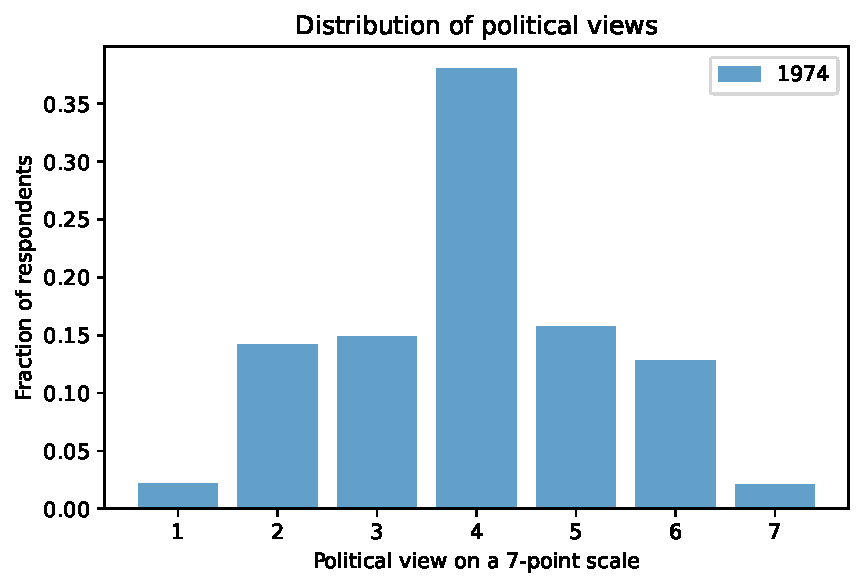
\includegraphics[width=4in]{chapters/02_polviews_files/02_polviews_32_0.pdf}
\end{center}

And from 2021:

\begin{lstlisting}[]
pmf21 = Pmf.from_seq(polviews21)
pmf21.bar(label="2021", color="C1", alpha=0.7)

decorate(
    xlabel="Political view on a 7-point scale",
    ylabel="Fraction of respondents",
    title="Distribution of political views",
)
\end{lstlisting}

\begin{center}
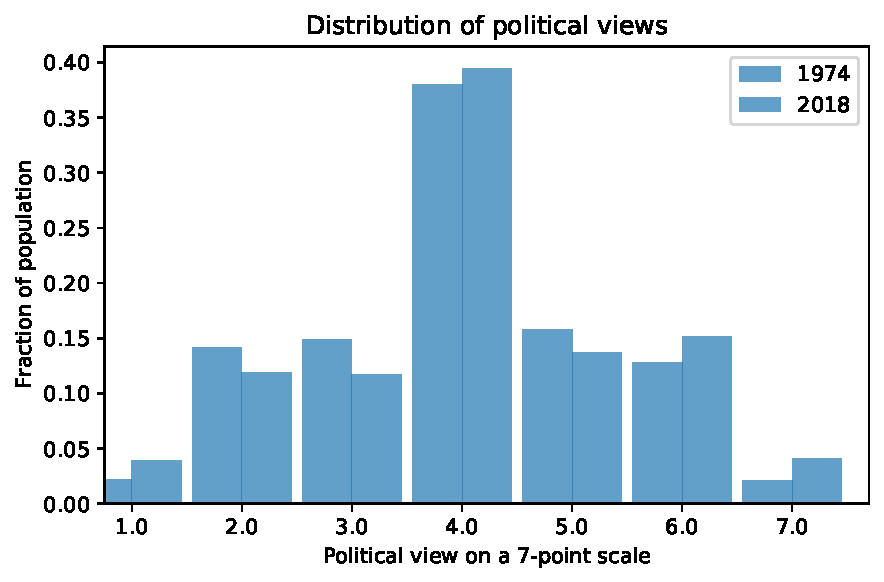
\includegraphics[width=4in]{chapters/02_polviews_files/02_polviews_34_0.pdf}
\end{center}

In both cases, the most common response is \passthrough{\lstinline!4!},
which is the code for ``moderate''. Few respondents describe themselves
as ``extremely'' liberal or conservative. So maybe we're not so
polarized after all.

\textbf{Exercise:} To summarize these changes, we can compare the mean
and standard deviation of \passthrough{\lstinline!polviews!} in 1974 and
2021.

The mean of the responses measures the balance of people in the
population with liberal or conservative leanings. If the mean increases
over time, that might indicate a shift in the population toward
conservatism.

The standard deviation measures the dispersion of views in the
population; if it increases over time, that might indicate an increase
in polarization.

Compute the mean and standard deviation of
\passthrough{\lstinline!polviews74!} and
\passthrough{\lstinline!polviews21!}.

What do they indicate about changes over this interval?

\hypertarget{plotting-a-time-series}{%
\section{Plotting a Time Series}\label{plotting-a-time-series}}

At this point we have looked at the endpoints, 1974 and 2021, but we
don't know what happened in between. To see how the distribution changed
over time, we can group by year and compute the mean of
\passthrough{\lstinline!polviews!} during each year. We can use
\passthrough{\lstinline!groupby!} to group the respondents by year.

\begin{lstlisting}[]
gss_by_year = gss.groupby("year")
gss_by_year
(@\dashfill@)
@@@<pandas.core.groupby.generic.DataFrameGroupBy object at 0x7f5d1c4f7c70>@@@
\end{lstlisting}

The result is a \passthrough{\lstinline!DataFrameGroupBy!} object that
represents a collection of groups.

In many ways the \passthrough{\lstinline!DataFrameGroupBy!} behaves like
a \passthrough{\lstinline!DataFrame!}. We can use the bracket operator
to select a column:

\begin{lstlisting}[]
polviews_by_year = gss_by_year["polviews"]
polviews_by_year
(@\dashfill@)
@@@<pandas.core.groupby.generic.SeriesGroupBy object at 0x7f5d5850e400>@@@
\end{lstlisting}

A column from a \passthrough{\lstinline!DataFrameGroupBy!} is a
\passthrough{\lstinline!SeriesGroupBy!}. If we invoke
\passthrough{\lstinline!mean!} on it, the results is a series that
contains the mean of \passthrough{\lstinline!polviews!} for each year of
the survey.

\begin{lstlisting}[]
mean_series = polviews_by_year.mean()
\end{lstlisting}

And here's what it looks like.

\begin{lstlisting}[]
mean_series.plot(color="C2", label="polviews")
decorate(xlabel="Year", ylabel="Mean (7 point scale)", title="Mean of polviews")
\end{lstlisting}

\begin{center}
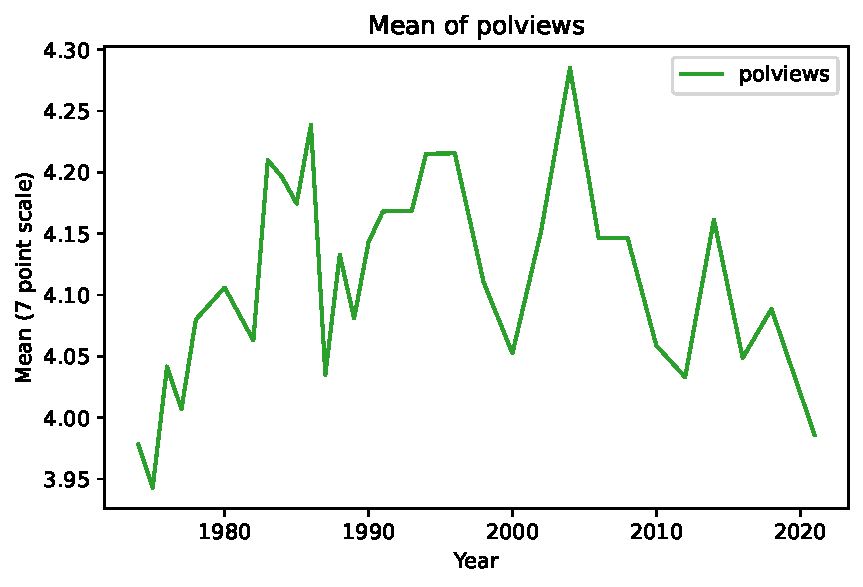
\includegraphics[width=4in]{chapters/02_polviews_files/02_polviews_50_0.pdf}
\end{center}

It looks like the mean increased between 1974 and 2000, decreased since
then, and ended up almost where it started. The difference between the
highest and lowest points is only 0.3 points on a 7-point scale, which
is a modest effect.

\begin{lstlisting}[]
mean_series.max() - mean_series.min()
(@\dashfill@)
@@@0.34240143126104083@@@
\end{lstlisting}

\textbf{Exercise:} The standard deviation quantifies the spread of the
distribution, which is one way to measure polarization. Plot standard
deviation of \passthrough{\lstinline!polviews!} for each year of the
survey from 1972 to 2021. Does it show evidence of increasing
polarization?

\hypertarget{smoothing-the-curve}{%
\section{Smoothing the Curve}\label{smoothing-the-curve}}

In the previous section we plotted mean and standard deviation of
\passthrough{\lstinline!polviews!} over time. In both plots, the values
are highly variable from year to year. We can use \textbf{local
regression} to compute a smooth line through these data points.

The following function takes a Pandas Series and uses an algorithm
called LOWESS to compute a smooth line. LOWESS stands for ``locally
weighted scatterplot smoothing''.

\begin{lstlisting}[]
from statsmodels.nonparametric.smoothers_lowess import lowess


def make_lowess(series):
    """Use LOWESS to compute a smooth line.

    series: pd.Series

    returns: pd.Series
    """
    y = series.values
    x = series.index.values

    smooth = lowess(y, x)
    index, data = np.transpose(smooth)

    return pd.Series(data, index=index)
\end{lstlisting}

We'll use the following function to plot data points and the smoothed
line.

\begin{lstlisting}[]
def plot_series_lowess(series, color):
    """Plots a series of data points and a smooth line.

    series: pd.Series
    color: string or tuple
    """
    series.plot(linewidth=0, marker="o", color=color, alpha=0.5)
    smooth = make_lowess(series)
    smooth.plot(label="", color=color)
\end{lstlisting}

The following figure shows the mean of
\passthrough{\lstinline!polviews!} and a smooth line.

\begin{lstlisting}[]
mean_series = gss_by_year["polviews"].mean()
plot_series_lowess(mean_series, "C2")
decorate(ylabel="Mean (7 point scale)", title="Mean of polviews", xlabel="Year")
\end{lstlisting}

\begin{center}
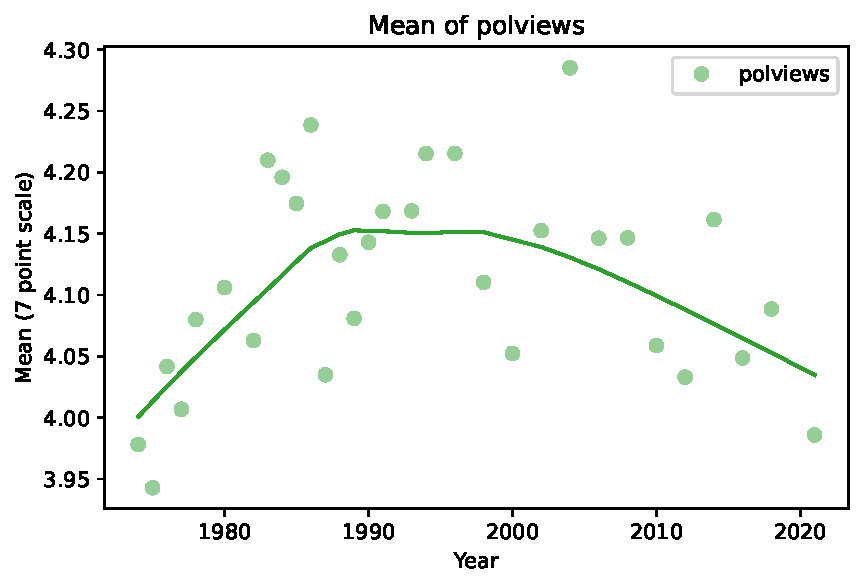
\includegraphics[width=4in]{chapters/02_polviews_files/02_polviews_59_0.pdf}
\end{center}

One reason the PMFs for 1974 and 2021 did not look very different is
that the mean seems to have gone up (more conservative) and then down
again (more liberal). Generally, it looks like the U.S. has been
trending toward liberal for the last 20 years, or more, at least in the
sense of how people describe themselves.

\textbf{Exercise:} Use \passthrough{\lstinline!plot\_series\_lowess!} to
plot the standard deviation of \passthrough{\lstinline!polviews!} with a
smooth line.

\hypertarget{cross-tabulation}{%
\section{Cross Tabulation}\label{cross-tabulation}}

In the previous sections, we treated \passthrough{\lstinline!polviews!}
as a numerical quantity, so we were able to compute means and standard
deviations. But the responses are really categorical, which means that
each value represents a discrete category, like ``liberal'' or
``conservative''. In this section, we'll treat
\passthrough{\lstinline!polviews!} as a categorical variable.
Specifically, we'll compute the number of respondents in each category
for each year, and plot changes over time.

Pandas provides a function called \passthrough{\lstinline!crosstab!}
that computes a \textbf{cross tabulation}, which is like a
two-dimensional PMF. It takes two \passthrough{\lstinline!Series!}
objects as arguments and returns a \passthrough{\lstinline!DataFrame!}.

\begin{lstlisting}[]
year = gss["year"]
column = gss["polviews"]

xtab = pd.crosstab(year, column)
\end{lstlisting}

Here are the first few lines from the result.

\begin{lstlisting}[]
xtab.head()
\end{lstlisting}

\begin{tabular}{lrrrrrrr}
\midrule
polviews &  1.0 &  2.0 &  3.0 &  4.0 &  5.0 &  6.0 &  7.0 \\
year &      &      &      &      &      &      &      \\
\midrule
1974 &   31 &  201 &  211 &  538 &  223 &  181 &   30 \\
1975 &   56 &  184 &  207 &  540 &  204 &  162 &   45 \\
1976 &   31 &  198 &  175 &  564 &  209 &  206 &   34 \\
1977 &   37 &  181 &  214 &  594 &  243 &  164 &   42 \\
1978 &   21 &  140 &  255 &  559 &  265 &  187 &   25 \\
\midrule
\end{tabular}

It contains one row for each value of \passthrough{\lstinline!year!} and
one column for each value of \passthrough{\lstinline!polviews!}. Reading
the first row, we see that in 1974, 31 people gave response 1,
``extremely liberal'', 201 people gave response 2, ``liberal'', and so
on.

The number of respondents varies from year to year, so we need to
normalize the results, which means computing for each year the
\emph{fraction} of respondents in each category, rather than the count.

\passthrough{\lstinline!crosstab!} takes an optional argument that
normalizes each row.

\begin{lstlisting}[]
xtab_norm = pd.crosstab(year, column, normalize="index")
\end{lstlisting}

Here's what that looks like for the 7-point scale.

\begin{lstlisting}[]
xtab_norm.head()
\end{lstlisting}

\begin{tabular}{lrrrrrrr}
\midrule
polviews &       1.0 &       2.0 &       3.0 &       4.0 &       5.0 &       6.0 &       7.0 \\
year &           &           &           &           &           &           &           \\
\midrule
1974 &  0.021908 &  0.142049 &  0.149117 &  0.380212 &  0.157597 &  0.127915 &  0.021201 \\
1975 &  0.040057 &  0.131617 &  0.148069 &  0.386266 &  0.145923 &  0.115880 &  0.032189 \\
1976 &  0.021877 &  0.139732 &  0.123500 &  0.398024 &  0.147495 &  0.145378 &  0.023994 \\
1977 &  0.025085 &  0.122712 &  0.145085 &  0.402712 &  0.164746 &  0.111186 &  0.028475 \\
1978 &  0.014463 &  0.096419 &  0.175620 &  0.384986 &  0.182507 &  0.128788 &  0.017218 \\
\midrule
\end{tabular}

Looking at the numbers in the table, it's hard to see what's going on.
In the next section, we'll plot the results.

\hypertarget{plotting-a-cross-tabulation}{%
\section{Plotting a Cross
Tabulation}\label{plotting-a-cross-tabulation}}

To see how the fraction of people with each political alignment has
changed over time, we'll use
\passthrough{\lstinline!plot\_series\_lowess!} to plot the columns from
\passthrough{\lstinline!xtab\_norm!}.

Here are the 7 categories plotted as a function of time. The
\passthrough{\lstinline!bbox\_to\_anchor!} argument passed to
\passthrough{\lstinline!plt.legend!} puts the legend outside the axes of
the figure.

\begin{lstlisting}[]
for name, column in xtab_norm.iteritems():
    plot_series_lowess(column, color_map[name])

decorate(
    xlabel="Year",
    ylabel="Proportion",
    title="Fraction of respondents with each political view",
)

plt.legend(bbox_to_anchor=(1.02, 1.02))
None
\end{lstlisting}

\begin{center}
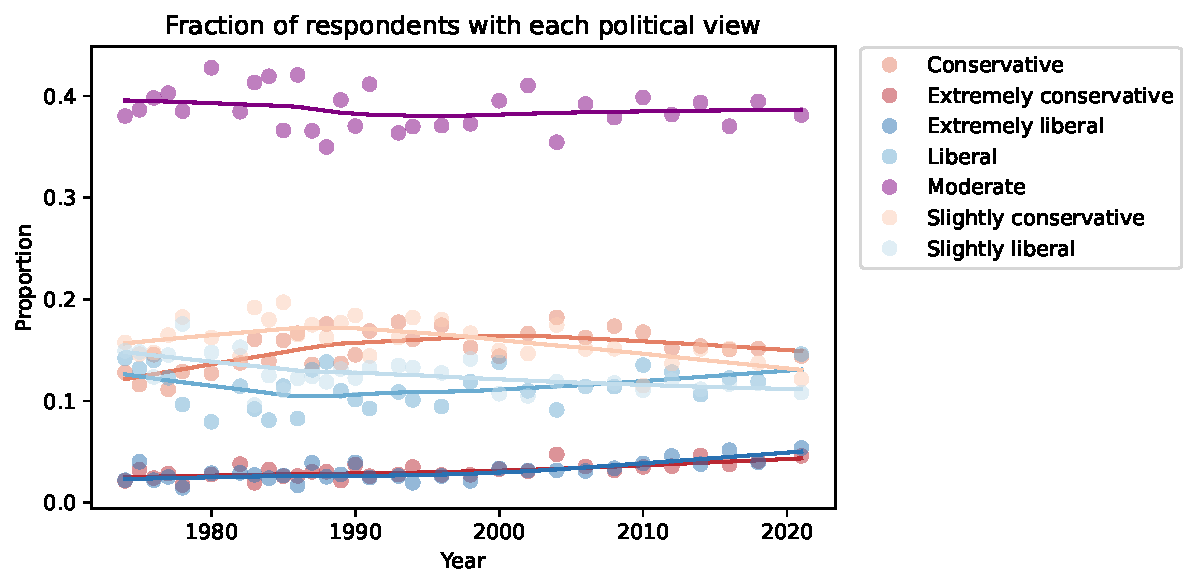
\includegraphics[width=4in]{chapters/02_polviews_files/02_polviews_88_0.pdf}
\end{center}

This way of looking at the results suggests that changes in political
alignment during this period have generally been slow and small. The
fraction of self-described moderates has not changed substantially. The
fraction of conservatives increased, but seems to be decreasing now; the
number of liberals seems to be increasing.

The fraction of people at the extremes has increased, but it is hard to
see clearly in this figure. We can get a better view by plotting just
the extremes.

\begin{lstlisting}[]
selected_columns = ["Extremely liberal", "Extremely conservative"]

for name, column in xtab_norm.iteritems():
    if name not in selected_columns:
        continue
    plot_series_lowess(column, color_map[name])

decorate(
    xlabel="Year",
    ylabel="Proportion",
    ylim=[0, 0.057],
    title="Fraction of respondents with extreme political views",
)
\end{lstlisting}

\begin{center}
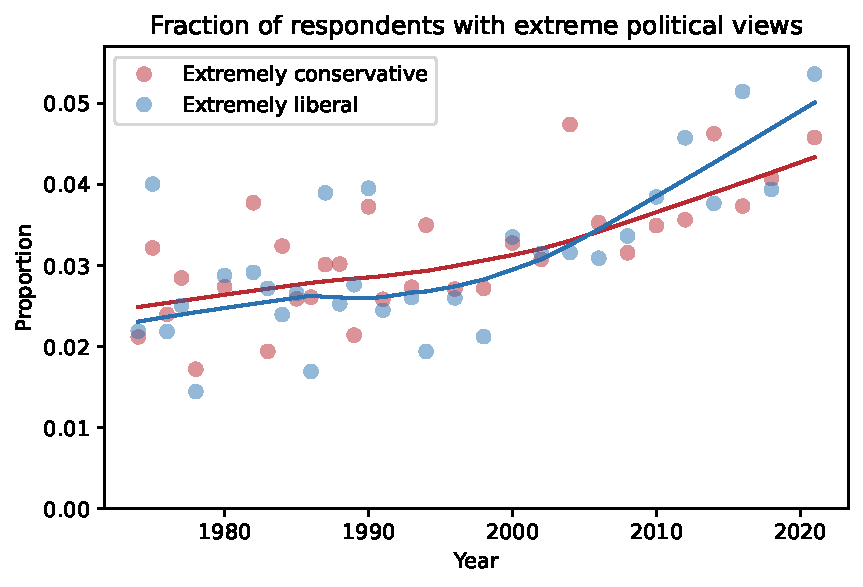
\includegraphics[width=4in]{chapters/02_polviews_files/02_polviews_90_0.pdf}
\end{center}

I used \passthrough{\lstinline!ylim!} to set the limits of the y-axis so
it starts at zero, to avoid making the changes seem bigger than they
are.

This figure shows that the fraction of people who describe themselves as
``extreme'' has increased from about 2.5\% to about 5\%. In relative
terms, that's a big increase. But in absolute terms these tails of the
distribution are still small.

\textbf{Exercise:} Let's do a similar analysis with
\passthrough{\lstinline!partyid!}, which encodes responses to the
question:

\begin{quote}
Generally speaking, do you usually think of yourself as a Republican,
Democrat, Independent, or what?
\end{quote}

The valid responses are:

\begin{lstlisting}
0   Strong democrat
1   Not str democrat
2   Ind,near dem
3   Independent
4   Ind,near rep
5   Not str republican
6   Strong republican
7   Other party
\end{lstlisting}

You can read the codebook for \passthrough{\lstinline!partyid!} at
\url{https://gssdataexplorer.norc.org/variables/141/vshow}. In the
notebook for this chapter, there are some suggestions to get you
started.

\hypertarget{summary}{%
\section{Summary}\label{summary}}

This chapter uses some tools we have seen before, like the
\passthrough{\lstinline!Pmf!} object and the
\passthrough{\lstinline!groupby!} function. And it introduces two new
tools: local regression for computing a smooth curve through noisy data,
and cross tabulation for counting the number of people, or fraction, in
each group over time.

Now that we have a sense of how political alignment as changed, in the
next chapter we'll explore the relationship between political alignment
and other beliefs and attitudes.

